% !TEX encoding = UTF-8
% !TEX TS-program = pdflatex
% !TEX root = ../tesi.tex

%**************************************************************
\chapter{Study case: AWS EC2 resources generation with Pulumi}
\label{cap:case-study}
%**************************************************************

\intro{Generation of AWS EC2 resources with Pulumi to compare how various languages supported by Pulumi will differ in the infrastructure resources declaration}\\

%**************************************************************
\section{Amazon Web Services}
AWS is a wide collection of services with many different purposes and characteristics including compute, storage, databases, analytics, networking, mobile, developer tools, management tools, IoT, security, and enterprise applications: on-demand, available in seconds, with pay-as-you-go pricing.
Anyway, for the purpose of the thesis we'll focus only on the EC2 module.

\subsection{AWS's EC2 module}
EC2 provides scalable computing capacity in the Amazon Web Services (AWS) Cloud.
Amazon EC2 eliminates the need to invest in hardware up front, so that the development and deployment of the applications is faster.
Such a characteristics is a perfect fit for an IaC scenario.

\section{Case study infrastructure overview}
For the thesis, only few components of the vast EC2 module have been selected to create a working infrastructure.\\
The infrastructure

\subsection{Components of the infrastructure}
The infrastructure we created for the case study of the thesis is an AWS EC2 \gls{VPC} hosting 3 private \gls{subnet}s, 3 public subnets, an \gls{internet gateway} to let the public subnets connect to the internet and a \gls{routing table} to map the public subnets to the internet gateway.
The architecture will look like the following:
\begin{center}
  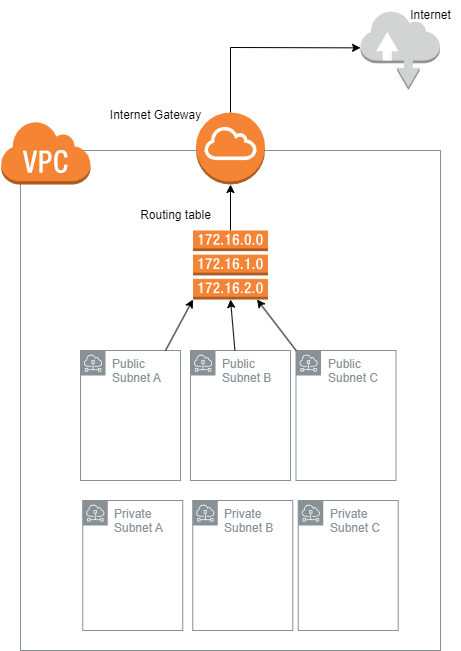
\includegraphics[width=1\columnwidth]{case_study/vpc_diagram} 
  \captionof{figure}{Infrastrutcture Architecture}
\end{center}\mbox{}\\
AWS is divided into regions, like us-east-1, eu-central-1, eu-south-1, etc.
For the purpose of our thesis eu-south-1 as a region has been chosen.
The servers of such a region are located in Milan.
Each region can have multiple availability zones, eu-south-1 has 3 different availability zones, and because of this we chose to create 3 couples of public/private subnets (A-A, B-B, C-C).
One couple on each availability zone.
The purpose of the availability zones is mainly for robustness.
If an availability zone becomes temporary unavailable, we can rely on the others to keep our services up.


\subsubsection{VPC}
The VPC is our "container" for all the other infrastructure resources.
We'll define within it the subnets, the internet gateway and the outing table.\\
The most important setting of our AWS EC2 VPC is the CIDR (Classless Inter-Domain Routing) block.
It represents the range of private IP addresses that the VPC can use to create and manage resources within the VPC.
\paragraph{CIDR}
The CIDR block is used to define the range of IP addresses that the VPC can use.
In our case the CIDR block is 10.136.0.0/24, which means that the VPC has access to all IP addresses from 10.136.0.0 to 10.136.0.255.
The 24 in the CIDR block is the prefix length, aka the subnet mask, that is used to identify the VPC.
The remaining 8 bits of the IP address will be used to identify the hosts in the VPC.\\
We'll assign a name as well to our VPC so that will be easier to recognize it when we'll inspect the AWS Management Console, that is the GUI version of the AWS CLI.

%val pvtSubnetsCidrs: List[String] = List("10.136.0.0/27", "10.136.0.32/27", "10.136.0.64/27")
%val pubSubnetsCidrs: List[String] = List("10.136.0.96/27", "10.136.0.128/27", "10.136.0.160/27")

\subsubsection{Subnet}
The subnets will require the ID of the VPC and the CIDR block that defines their IP scope.
For the subnets we'll use the following CIDR blocks:
\begin{itemize}
  \item Private Subnet A: 10.136.0.0/27
  \item Private Subnet B: 10.136.0.32/27
  \item Private Subnet C: 10.136.0.64/27
  \item Public Subnet A: 10.136.0.96/27
  \item Public Subnet B: 10.136.0.128/27
  \item Public Subnet C: 10.136.0.160/27
\end{itemize}
3 of the 8 bits left out for the hosts identification have been used to identify the subnets.
In fact we shall notice that now the subnet mask is not 24 anymore, but 27.
Hence, we are left with 5 bits to identify the hosts within each subnet, giving us 32 possible IPs.
From such IPs 2 are reserved for the network address and the broadcast address, so we have 30 possible IPs.
We won't discuss this topic any further since it isn't essential for the final objective of the thesis.\\
Moreover, we'll define also the availability zone for each subnet.


\subsubsection{InternetGateway}
The definition of the internet gateway is actually quite straight forward.
The mandatory parameter to assign is the ID of the VPC.

\subsubsection{RouteTable}
\label{sssec:routetable}
The definition of a route table is required in order to bind the public subnets to the internet gateway, so that they can send and receive data over the internet.\\
Here, along with the VPC ID, we assign the routes of such routing table.
In order to do this we have to provide a CIDR and a target resource to which the packet will be forwarded to, that can be a subnet or the internet gateway in our case.
The internet gateway is mapped with the CIDR block 0.0.0.0/0.
Obviously also the ID of the internet gateway is required in order to bind it to the routing table.\\
In a nutshell this means that every packet not directed to a host within the VPC will be routed to the internet gateway and then to the internet.\\
The association of the public subnets to the routing table will be achieved using the \textit{route table association} resource.
Such a resource will require us to provide the id of the subnet and the id of the routing table to establish a connection.
The private subnets will not be associated to such a routing table, since we want to keep them private.
Differently, without explicitly associating them to a given routing table, AWS will automatically associate them to a default routing table that, being not bound to an internet gateway, will keep them private.\\


\section{Typescript implementation of the case study}
\label{sec:typescript-impl}
The first version of the implementation of the previously defined architecture is written using the Typescript APIs of Pulumi.
The structure of the project, and this holds for the Java and Scala version as well, is trivial.
We have a simple \texttt{index.ts} file that defines the entry point for our typescript project, and it is just a couple of lines long:
\begin{lstlisting}[numbers=left, numberstyle=\tiny, numbersep=-5pt, stepnumber=1]
  import { VPC } from './VPC/VPC';

  const vpc = new MyVPC("Custom VPC");
\end{lstlisting}\mbox{}\\
The interesting part relies on the \texttt{MyVPC} class.
Such a class extends the \texttt{ComponentResource} class of Pulumi.
In our typescript implementation, we use the constructor of the user-defined \texttt{MyVPC} class to call all the class methods that are responsible for the creation of the resources.
But this is just mentioned since the interesting part of the code are the actual methods that are responsible for the creation of the resources.

\subsection{VPC resource creation}
The code to the VPC resource creation API of Pulumi is done in this method of the \texttt{MyVPC} class:
\begin{lstlisting}[numbers=left, numberstyle=\tiny, numbersep=-5pt, stepnumber=1]
  protected createVPC() {
    this.vpc = new Vpc("vpc\_res", {
      cidrBlock: "10.136.0.0/24",
      tags: {
        Name: "myVPC-typescript",
      },
    },
    {
      parent: this,
    });
  }
\end{lstlisting}\mbox{}\\
\texttt{vpc\_res} is the name that will be given by Pulumi at this resource once on the stack.
We can notice how the various parameters are given in a declarative style within the curly brackets.
Such a syntax is syntactic sugar for a Map definition.\\
At line 8 the parent of this resource is set.
With this specification, we are telling to the stack of Pulumi that the vpc resource \texttt{vpc\_res} that we are creating is a child resource of the VPC resource identified by the \texttt{MyVPC} class.

\subsection{Internet gateway creation}
To create the internet gateway resource we can use the following code:
\begin{lstlisting}[numbers=left, numberstyle=\tiny, numbersep=-5pt, stepnumber=1]
  protected createIGW(){
    this.gw = new InternetGateway("gw", {
      vpcId: this.vpc?.id,
      tags: {
          Name: "myIGW-typescript",
      },
    },
    {
      parent: this.vpc,
    });
  }
\end{lstlisting}\mbox{}\\
It is really simple since it requires just the ID of the VPC in which it has to be created and optionally a name and a parent for the Pulumi's stack representation.


\subsection{Subnets creation}
To create the private and the public subnets we require a more complex logic.
The function that has been used is \texttt{protected createAZsSubnets(isPvt: Boolean)}.
It is called twice, once with a true value to create the private subnets, and another one with false to instantiate the public ones (and connect them to the routing table bound with the internet gateway).\\
In the body of the function, first we want to get all the availability zones present in the AWS region we are working on.
To achieve this, we will use such a function \texttt{this.availableZones = aws.getAvailabilityZonesOutput()}.\\
Second, we want to create both a private and public subnet in each availability zone acquired with the aforementioned method.
The \texttt{pulumi.all} function, in combination with the \texttt{apply} function will help us in achieving such a goal.\\

\subsubsection{pulumi.all}
\label{sssec:pulumi-all}
\texttt{pulumi.all} is a utility function in Pulumi that allows you to combine multiple Outputs into a single Output that resolves to an array of the resolved values of each Output.
So if we consider the following code:
\begin{lstlisting}[numbers=left, numberstyle=\tiny, numbersep=-5pt, stepnumber=1]
  pulumi.all([this.availableZones.names, this.vpc!.id])
\end{lstlisting}\mbox{}\\
Such a call returns us an \texttt{Output<[string[], string]>}.
The array of strings is the list of the availability zones names, while the second string represents the ID of our VPC on AWS EC2.
Now we have a new Output type that is more suitable to create the subnets based on our VPC ID, because the function apply is letting us "open" an \texttt{Output} value and access its content.

\subsubsection{.apply}
Lets extend our code in this way:
\begin{lstlisting}[numbers=left, numberstyle=\tiny, numbersep=-5pt, stepnumber=1]
  pulumi.all([this.availableZones.names, this.vpc!.id]).apply(([azNames, vpcId]) => {
    // lambda's body to create the subnets here
  })
\end{lstlisting}\mbox{}\\
The apply function is letting us access \texttt{Output<[string[], string]>} and apply some logic on the inner values.\\

\paragraph{The apply's lambda}
\label{par:ts-lambda}
Now that we have the access to the list of availability zones and the VPC ID, we can iterate over the availability zones and create the subnets for our VPC.
Here is the complete code of the function:
\begin{lstlisting}[numbers=left, numberstyle=\tiny, numbersep=-5pt, stepnumber=1]
  protected createAZsSubnets(isPvt: Boolean) : Output<Subnet[]>{
    this.availableZones = aws.getAvailabilityZonesOutput()
    return pulumi.all([this.availableZones.names, this.vpc!.id]).apply(([azNames, vpcId]) => {
      let i = 0
      let listToPushInto: Subnet[] = Array<aws.ec2.Subnet>()
      azNames.forEach(azName => {
        let fullName = azName + (isPvt ? "-pvt" : "-pub") + "-subnet-typescript"
        listToPushInto.push(new Subnet(fullName, {
          vpcId: vpcId,
          availabilityZone: azName,
          cidrBlock: isPvt ? this.pvtSubnetsCidrs[i] : this.pubSubnetsCidrs[i],
          tags: {
            Name: fullName,
          },
        },{
          parent: this.vpc
        }));
        i++;
      });
      return listToPushInto
    });
  }
\end{lstlisting}\mbox{}\\
In the code we instantiate private or public public subnets basing on the \texttt{isPvt} passed in the \texttt{createAZsSubnets}.
We can notice that for the creation of a subnet we pass arguments such as \texttt{vpcId}, the availability zone name, the CIDR block, and a name (that is a tag) to better identify it on the stack.\\
Each newly created subnet is then pushed into the class field \texttt{this.prvSubNets} or \texttt{this.pubSubNets} (that are arrays of subnets), basing on the nature of the subnet.\\
The creation of a subnet requires us to provide both the availability zone name and the ID of the VPC.
Since these two pieces of information are contained in two separate \texttt{Output}s (\texttt{Output<String[]>} and \texttt{Output<String>} respectively) we must first use the \texttt{pulumi.all} to wrap them in a single \texttt{Output<String[], String>}.
This due to the fact that \texttt{.apply} can accept a single \texttt{Output<A>}, for any \texttt{A} type, value as input and not a pair.
Then, we can use the \texttt{.apply} to unbox from the \texttt{Output<String[], String>} its inner value.
Now that we have both the pieces of information out of the context value, we can use them to create the subnets.\\
%The \texttt{this.pubSubNets} will be used by the \texttt{this.attachRouteTableToPubSubnets()} function to bind the public subnets to the internet gateway through the routing table.\\
%The crucial point here is that in order to bind the public subnets to the routing table, we must call \texttt{this.attachRouteTableToPubSubnets()} as the last step in our \texttt{pulumi.all} function call.
%This ensures that we have all the necessary subnets to make the binding, since the call will be done at the completion of the creation of the subnets.
We can notice that the \texttt{.apply} function is, at the end of its lambda function, returning a list of the created subnets.
Such a return is also the return of the function and is indeed of the \texttt{Output<Subnet[]>} type.

\subsection{Routing table creation}
This is the code to create the routing table resource:
\begin{lstlisting}[numbers=left, numberstyle=\tiny, numbersep=-5pt, stepnumber=1]
  protected createRouteTable() {
    this.routeTable = new RouteTable("example", {
      vpcId: this.vpc!.id,
      routes: [
          {
              cidrBlock: "0.0.0.0/0",
              gatewayId: this.gw!.id,
          },
      ],
      tags: {
          Name: "myRouteTable-typescript",
      },
  },
  {
    parent: this.vpc,
  });
  }
\end{lstlisting}\mbox{}\\
On top of the classic VPC ID we are assigning here the routes.
As we mentioned before in the \hyperref[sssec:routetable]{Routetable} paragraph, we are defining the route with CIDR 0.0.0.0/0 to redirect all the packets coming from the public subnets, and not having as destination an IP internal at our VPC, to the internet gateway.\\
We are also giving a name to the routing table and assigning its parent.


\subsection{Attaching the public subnets to the internet gateway}
As we mentioned previously, we use the \texttt{this.attachRouteTableToPubSubnets()} function to attach the public subnets to the internet gateway.
Here is the code of the function:
\begin{lstlisting}[numbers=left, numberstyle=\tiny, numbersep=-5pt, stepnumber=1]
  protected attachRouteTableToPubSubnets(){
    let i = 0
    this.pubSubNets.apply(subNets => {
      subNets.forEach(sn => {
        new aws.ec2.RouteTableAssociation(`${i}-routeTableAssociation-typescript`, {
          subnetId: sn.id,
          routeTableId: this.routeTable!.id,
        },
        {
          parent: this.vpc
        });
        i++
      })
    });
  }
\end{lstlisting}\mbox{}\\
Here we used once more, as for the subnets creation, a combination of \texttt{.apply} and a foreach to iterate over all the extracted subnets (\texttt{.foreach}) from the Output context (\texttt{.apply}).\\
Inside the \texttt{foreach}'s lambda we are defining a new \texttt{RouteTableAssociation} AWS EC2 resource that requires just the id of the subnet and the id of the routing table to which we want to attach the subnet to.

\section{Creating the resources with Pulumi}
After having seen all the code to create the resources, we'll see what the Pulumi command \texttt{pulumi up} will do.
The command checks if all the resources that we want to create have valid parameters and there are not circular dependencies among the resources on their creation.
If everything is nice and neat, it will shows us the preview of the changes that we are about to get:
\begin{center}
  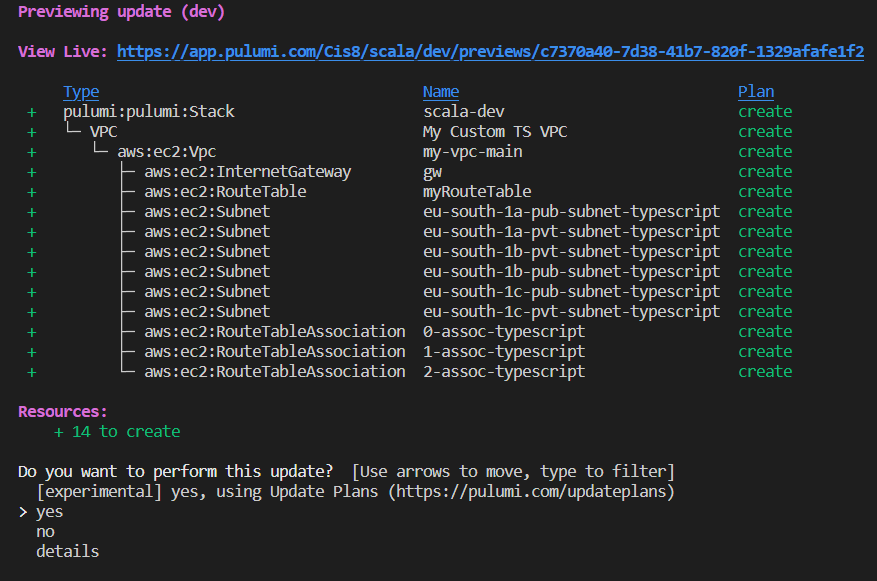
\includegraphics[width=1\columnwidth]{case_study/pulumi_up_1} 
  \captionof{figure}{pulumi up preview}
\end{center}\mbox{}\\

If we press yes this is the output:
\begin{center}
  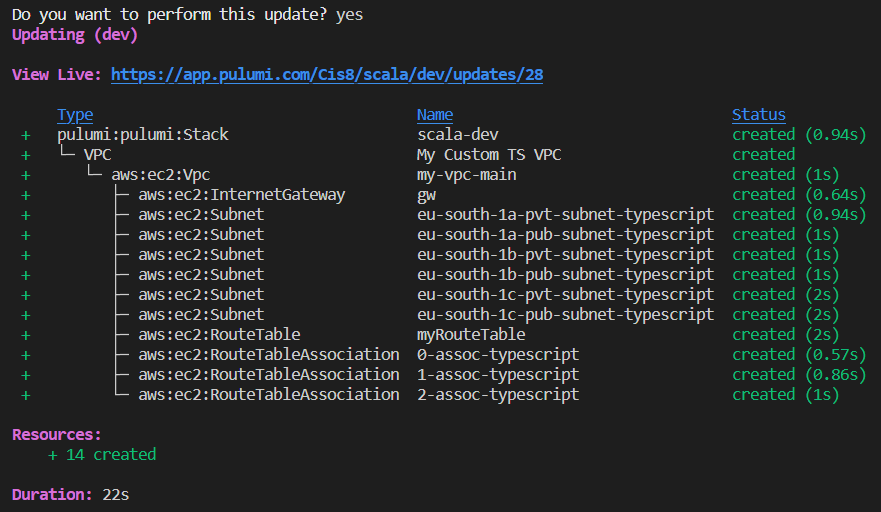
\includegraphics[width=1\columnwidth]{case_study/pulumi_up_2} 
  \captionof{figure}{pulumi up confirmed}
\end{center}\mbox{}\\
We can notice how the resources created are nested into each other thanks to the parent option that we used.
This is helping us in keeping our resources on the stuck nicely ordered and tied up.\\

\section{Destroying the resources with Pulumi}
Now lets use the \texttt{pulumi destroy} command to destroy the resources on our Pulumi's stack.
The preview of the changes that we are about to get look like this:
\begin{center}
  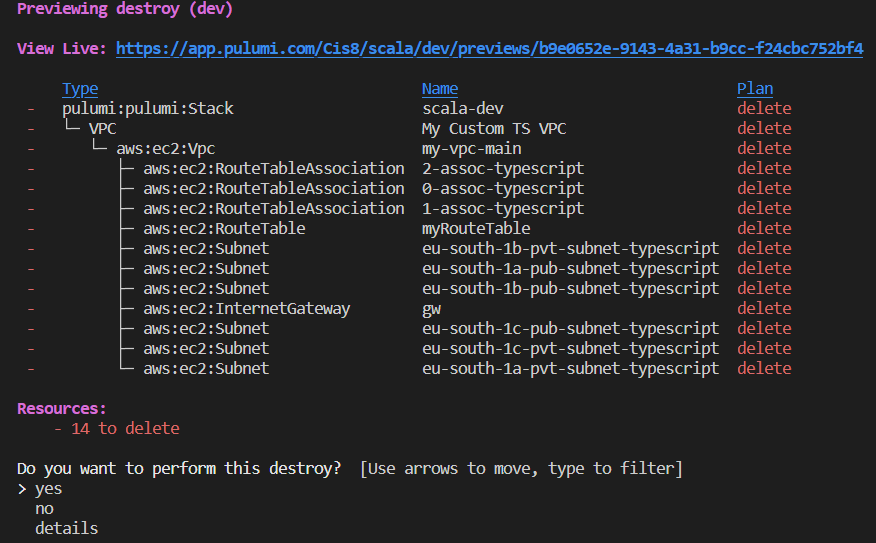
\includegraphics[width=1\columnwidth]{case_study/pulumi_destroy_1} 
  \captionof{figure}{pulumi destroy preview}
\end{center}\mbox{}\\

If we confirm the changes this is the result:
\begin{center}
  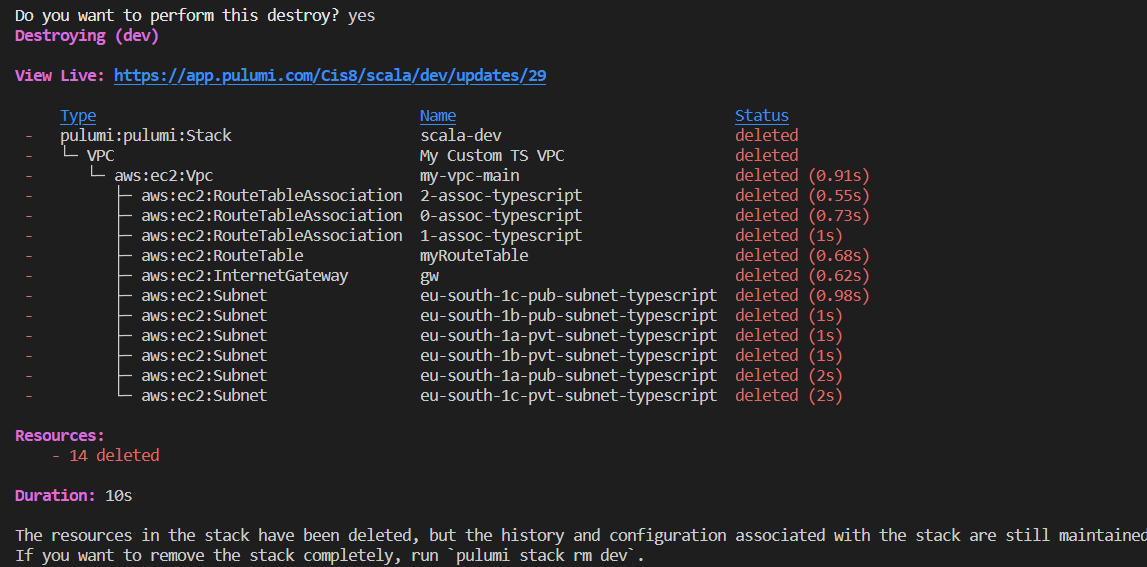
\includegraphics[width=1\columnwidth]{case_study/pulumi_destroy_2} 
  \captionof{figure}{pulumi destroy confirmed}
\end{center}\mbox{}\\

%\section{Java implementation of the case study}

\section{My Scala implementation of the case study}
Since Scala is not supported by Pulumi, I had to implement it on my own.
The Pulumi team is clear on the official way to add the support of a new language for Pulumi, and the procedure is long and laborious, too laborious for a master thesis.
The full procedure can be found on \href{https://github.com/pulumi/pulumi/wiki/New-Language-Bring-up}{New Language Bring Up}.\\
The idea behind the adopted solution is to exploit the compatibility of Scala with the Java libraries to write custom syntactic sugar.
Such syntactic sugar will be based on the Pulumi Java's APIs and will provide to the user cool constructs to write readable and expressive code to interact with Pulumi.\\
The steps of the work done have been the followings:
\begin{enumerate}
  \item manually write the \textit{sugarized} functions to create the Pulumi resources using Scala
  \item use such functions to recreate the Stack obtained with the typescript solution shown before in the \hyperref[sec:typescript-impl]{Typescript implementation of the case study} section
  \item create an automatic code generator for our syntactic sugar functions, so that we can quickly create a library for Scala's Pulumi APIs
  \item try to recreate the stack with the automatically generated code
\end{enumerate}
Obviously, the third step is quite wide, and if fact with my work I had the time to generate only the functions for a part of the Java's Pulumi APIs for the AWS EC2 module.\\
Now the just defined steps will more accurately presented.

\subsection{Structure of the Java APIs for the constructors of the resources in Pulumi}
To understand the syntactic sugar functions that I defined, let's first consider the general structure of the Java APIs for the constructors of the resources.\\
The constructor of a resource, in general accepts a name and an instance of the corresponding \texttt{Args} class of the resource we are creating.
Lets consider for example the Vpc resource.
In Java, to instantiate such a resource we'd call:
\begin{lstlisting}[numbers=left, numberstyle=\tiny, numbersep=-5pt, stepnumber=1]
  protected Vpc vpc = new Vpc("my-vpc-java", VpcArgs.builder()
    .cidrBlock("10.136.0.0/24")
    .tags(Map.of("Name", "main"))
    .build(),
          CustomResourceOptions.builder()
                  .parent(this)
                  .build());
\end{lstlisting}\mbox{}\\
We can (hardly) see that along with the name to be assigned to the vpc "my-vpc-java", a VpcArgs builder and a CustomResourceOptions builder are passed by.
These builders will create an instance of the respective classes that will be used to set respectively the parameters and the parent of the Vpc resource.
So, for our case study we need to consider: the name to be assigned at the created resource on the Pulumi stack, the builder of the respective \texttt{Args} class of the resource, and the \texttt{CustomResourceOptions} builder.


\subsection{Syntactic sugar usage}
\label{ssec:syn-sug-usage}
Our syntactic sugar is split in 2 categories of functions.
The first is about the functions that represent the constructors of the resources.
The second is for the methods available within the builders of the \texttt{Args} classes and for the CustomResourceOptions builder functions.
The idea to create a resource is to call the \textit{sugarized} function that represent the constructor of that resource, and and then call the Builder methods to assign the various parameters to the resource.

\subsubsection{Vpc creation}
\label{sssec:vpc-creation-scala}
This is how a Vpc resource can be created with my syntactic sugar:
\begin{lstlisting}[numbers=left, numberstyle=\tiny, numbersep=-5pt, stepnumber=1]
  val myVpc = vpc("scala-main") ({
    cidrBlock("10.136.0.0/24")
    tags("Name" -> "myVpcScala")
  },{
    parent(this)
  })
\end{lstlisting}\mbox{}\\
At line 1, the \texttt{vpc} function is the actual \textit{sugarized} function for the VPC resource constructor.
In fact we can notice that we have a curried function.
The first parentheses is taking the parameter for the resource name on the Pulumi stack, while the second one is containing two lambdas (defined by the curly brackets).
These lambdas are respectively used to call all the builder methods of the \texttt{VcpArgs} class and the ones for the \texttt{CustomResourceOptions}.\\
We can notice that we didn't explicitly defined an instance of the builders of such classes.
We will soon see how we achieved such a syntactic sugar trick.\\
The \texttt{cidrBlock} and the \texttt{tags} methods are the generated methods for builder of the \texttt{VpcArgs} class.\\ 
The \texttt{parent} method instead is the generated method for the builder of the \texttt{CustomResourceOptions} class.\\
Moreover, we can also notice that inside tags, that expects a \texttt{Map[String, String]} type, the instantiation of a \texttt{Map[String, String]} containing a single elements isn't required.
This other trick will be explained later as well.

\subsubsection{Internet gateway creation}
Much similar to the VPC resource, we have this code for the internet gateway creation:
\begin{lstlisting}[numbers=left, numberstyle=\tiny, numbersep=-5pt, stepnumber=1]
  val myIGW = internetGateway("gw") ({
    vpcId(myVpc.getId())
    tags("Name" -> "myIGWScala")
  },{
    parent(myVpc)
  })
\end{lstlisting}\mbox{}\\
The code won't be commented since is analogous to the VPC case.

\subsubsection{Routing table creation}
\label{sssec:routetable-creation-scala}
The code to create a routing table:
\begin{lstlisting}[numbers=left, numberstyle=\tiny, numbersep=-5pt, stepnumber=1]
  val myRouteTable = routeTable("myRouteTable") ({
    vpcId(myVpc.getId())
    routes(
      routeTableRouteArgs(){
        cidrBlock("0.0.0.0/0")
        gatewayId(myIGW.getId())
      })
    tags("Name" -> "myRouteTableScala")
  },{
    parent(myVpc)
  })
\end{lstlisting}\mbox{}\\
The only thing that is worth to mention here is that the \texttt{routes} function, at line 3, expects a \texttt{List[RouteTableRouteArgs]}, but we are providing only a \texttt{RouteTableRouteArgs}.
As for the case of the \texttt{Map[String, String]} with the parent method mentioned above, the same trick has been used to provide syntactic sugar that lifts us from the need of instantiate a singleton \texttt{List[RouteTableRouteArgs]} manually.

\subsubsection{Subnets creation}
\label{sssec:subnets-creation}
Much different from the other resources is the function to create the subnets:
\begin{lstlisting}[numbers=left, numberstyle=\tiny, numbersep=-5pt, stepnumber=1,linewidth=420pt]
  def createAzSubnets(isPvt: Boolean) =
    availabilityZonesNames().map((az: GetAvailabilityZonesResult) =>
      for
        (name, cidr) <- az.names().zip(if isPvt then pvtSubnetsCidrs else pubSubnetsCidrs)
      yield
        val fullName = name + "-" + (if isPvt then "pvt" else "pub") + "-subnet-scala"
        subnet(fullName) ({
          vpcId(myVpc.getId())
          availabilityZone(name)
          cidrBlock(cidr)
          tags("Name" -> fullName)
        },{
          parent(myVpc)
        })
    )
\end{lstlisting}\mbox{}\\
We can notice here how we had the possibility to use the \texttt{map} function on \texttt{availabilityZonesNames()}.
\texttt{availabilityZonesNames()} returns a \texttt{Output[GetAvailabilityZonesResult]} value, that isn't directly accessible from the \texttt{map} function.
To achieve such a result we made a monad out of the \texttt{Output} type, so that map can be applied on the inner value of the \texttt{Output} context.
We'll see better how is the actual implementation of the monad soon.\\
The for yield construct here is iterating over a zipped list made out of the availability zones names and the CIDR blocks for the respective kind of subnet to create (private or public, based on the input parameter isPvt).
The for yield, for each tuple \texttt{(name, cidr)} will create a \texttt{Subnet} value and will return a \texttt{Subnet[]} as output.
Now, the for is still inside the lambda of the \texttt{availabilityZonesNames().map} function.
Consider the fact that \texttt{map} takes an \texttt{Output[A]} and returns an \texttt{Output[B]}, where \texttt{A = GetAvailabilityZonesResult} and \texttt{B = Output[Iterable[Subnet]]}.
This is different from the typescript implementation in the \hyperref[par:ts-lambda]{Apply's lambda} paragraph, where the function that creates the subnets returns a plain \texttt{Subnet[]}.\\
We will make further considerations about such a difference in the \hyperref[cap:comparisons]{Comparison between the languages for Pulumi and the advantages of Scala} chapter.\\

\subsubsection{Attaching the subnets to the routing table}
\begin{lstlisting}[numbers=left, numberstyle=\tiny, numbersep=-5pt, stepnumber=1]
  def attachRouteTableToPubSubnets(): Output[Iterable[RouteTableAssociation]] =
    pubSubnets.map((subnets: Iterable[Subnet]) =>
        for
          (ps, idx) <- subnets.zipWithIndex
        yield
          routeTableAssociation(idx + "-assoc-scala") ({
            subnetId(ps.getId())
            routeTableId(myRouteTable.getId())
          }, {
            parent(myVpc)
          })
      )
\end{lstlisting}\mbox{}\\
Similarly to the subnet creation function, also here we use map to "unbox" an \texttt{Output[Iterable[Subnet]]} value, to apply some logic on the inner value and then return a \texttt{Output[Iterable[RouteTableAssociation]]} value as result.
Since the logic is analogous we won't comment this code further, but the fact we're having these two functions that both take an Output[A] as input and return an Output[B] will be a key point for our observations in the \hyperref[cap:comparisons]{Comparison between the languages for Pulumi and the advantages of Scala} chapter.

\subsubsection{Resources creation with pulumi up}
\label{sssec:res-cre-ts}
Now lets make sure that the stack created with \texttt{pulumi up} is the same of the one created with the typescript implementation.
From this image we can see that they are equivalent to the ones shown in \hyperref[sssec:res-cre-ts]{Resources creation with pulumi up in Typescript}:
\begin{center}
  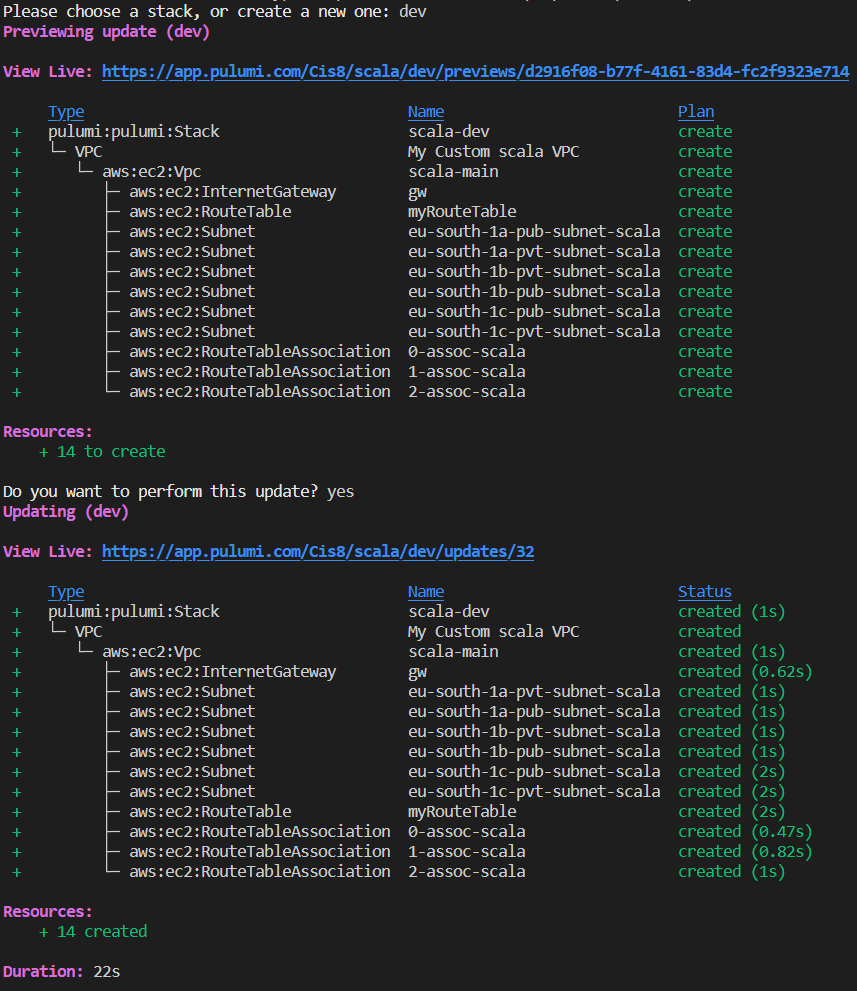
\includegraphics[width=1\columnwidth]{case_study/pulumi_up_scala_result} 
  \captionof{figure}{pulumi up result with the scala implementation}
\end{center}\mbox{}\\

\subsection{Syntactic sugar for the constructors of the resources}
All the methods that we just used for creating the Pulumi resources in Scala (\texttt{vpc, internetGateway}, ecc.), behind the scenes are implemented following a common pattern.
Consider the vpc function of the syntactic sugar defined inside the "PulumiUtilFunctionsForScala.scala" file:
\begin{lstlisting}[numbers=left, numberstyle=\tiny, numbersep=-5pt, stepnumber=1]
  def vpc(param: String)
         (init: VpcArgs.Builder ?=> Unit,
          initOpt: (CustomResourceOptions.Builder ?=> Unit) = baseOpts): Vpc =
	  given b: VpcArgs.Builder= VpcArgs.builder()
	  init
	  given bo: CustomResourceOptions.Builder = CustomResourceOptions.builder()
	  initOpt
	  new Vpc(param, b.build(), bo.build())
\end{lstlisting}\mbox{}\\
Lets analyze the function by steps.
First of all we can see that the function declaration is curried, we have 2 parentheses with different input parameters.\\
The first parentheses take simply a string parameter, that is used to set the name of the \texttt{Vpc} resource on the Pulumi stack.\\
The second parentheses are taking two lambdas as parameters: a \texttt{VcpArgs.Builder ?=> Unit}  and a \texttt{CustomResourceOptions.Builder ?=> Unit}, with default parameter baseOpts, that we'll see in a moment what is.\\
In Scala, a lambda that takes an Int and returns a String has this type notation: \texttt{Int => String}, so does that '\texttt{?}' in front of the '\texttt{=>}' mean?\\
Such '\texttt{?=>}' is denoting a context function, that is a function with (only) context parameters.
In the \hyperref[par:given-using]{Given and using keywords} paragraph we introduced the \texttt{using} keyword.
Such '\texttt{?}' is quite analogous to a \texttt{using} keyword used to mark an function's input parameter as a context parameter.
This is, in part, what let us call the builder methods like \texttt{cidrBlock("10.136.0.0/24")} and \texttt{tags("Name" -> "myVpcScala")} (as shown in the code shown in the \hyperref[sssec:vpc-creation-scala]{Vpc creation in Scala} paragraph)
without having to call them on a specific builder instance.
We will get the whole picture of this trick when we'll talk about the syntactic sugar for the builder methods in the \hyperref[ssec:syn-sug-builders]{Syntactic sugar for the builders' methods} paragraph.

\subsubsection{Correspondence between the input parameters and the user defined code used to create the VPC}
To have a better idea to what these parameters refer in our VCP creation case, consider this image:
\begin{center}
  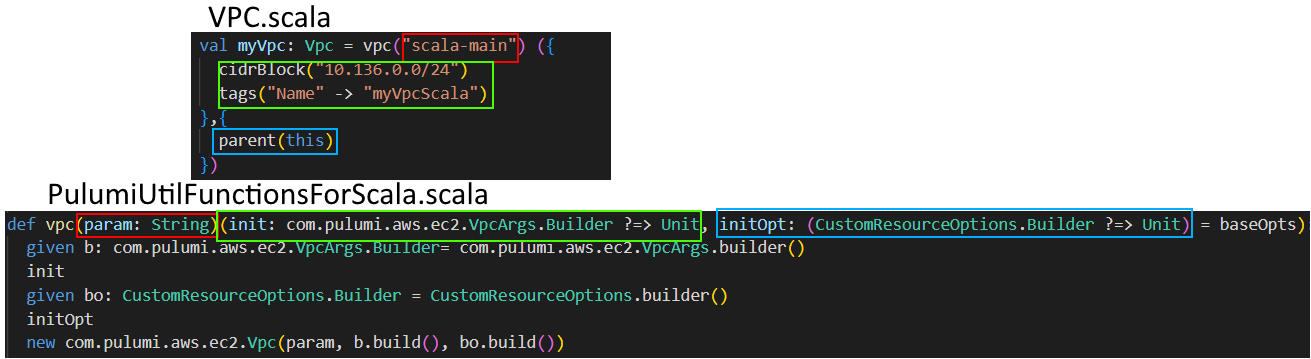
\includegraphics[width=1.3\columnwidth]{case_study/vpc_params_boxes} 
  \captionof{figure}{Parameters correspondence}
\end{center}\mbox{}\\
The red box represents the name for our VPC resource on the Pulumi stack.\\
The green one, with the curly brackets, is the lambda that takes a \textit{given} \texttt{VpcArgs.Builder} as an implicit parameter from the context.
In fact we are not providing any explicitly.
The \texttt{given b} defined in the first line of the body of the \texttt{vpc} function is the instantiation of a \textit{given} instance of such a builder, that will be automatically injected by the compiler in the \texttt{init} lambda represented by the green box.\\
Analogous is the concept for the blue box.\\

\subsubsection{Vpc construction}
Now that we understood what are the input parameters of our \texttt{vpc} function and to what do they correspond in the resource creation shown in the \hyperref[ssec:syn-sug-usage]{Syntactic sugar usage} section, we can see how the actual creation of the resource is made.
After having executed the \texttt{init} and \texttt{initOpt} lambdas, that behind the scenes will set the parameters of the respective \textit{given} builders, we can create the resource using the constructor offered by the Pulumi Java APIs.
\texttt{new Vpc(param, b.build(), bo.build())} is a direct call to such libraries, and will create actually create the \texttt{VPC}.

\subsubsection{The baseOpts function}
The \texttt{baseOpts} function that we mentioned before as a default lambda for our \texttt{vpc} function is the following:
\begin{lstlisting}[numbers=left, numberstyle=\tiny, numbersep=-5pt, stepnumber=1]
  def baseOpts(using o: CustomResourceOptions.Builder) : Unit = {}
\end{lstlisting}\mbox{}\\
In practice, is an vacuous lambda that does nothing on the \texttt{CustomResourceOptions} builder.
The question here is: \textit{why do we need such a default function?}
To answer the question let's consider one more time the code to create a VPC with out syntactic sugar:
\begin{lstlisting}[numbers=left, numberstyle=\tiny, numbersep=-5pt, stepnumber=1]
  val myVpc: Vpc = vpc("scala-main") ({
    cidrBlock("10.136.0.0/24")
    tags("Name" -> "myVpcScala")
  },{
    parent(this)
  })
\end{lstlisting}\mbox{}\\
We can see that we passed both the lambdas for the \texttt{VpcArgs} builder and for the \texttt{CustomResourceOptions} builder, but what if we want to simply use the \texttt{VpcArgs} builder and not set the parent?
We can do the following:
\begin{lstlisting}[numbers=left, numberstyle=\tiny, numbersep=-5pt, stepnumber=1]
  val myVpc: Vpc = vpc("scala-main") {
    cidrBlock("10.136.0.0/24")
    tags("Name" -> "myVpcScala")
  }
\end{lstlisting}\mbox{}\\
This code compiles, and we can notice that we even got rid of the parentheses around the two groups of curly brackets for the lambdas.
If this compiles is only thanks to the default parameter that is automatically injected in by the compiler, as we didn't give an explicit one.\\
Another question now might arise: \textit{why didn't we change the signature of the function in the following way?}
\begin{lstlisting}[numbers=left, numberstyle=\tiny, numbersep=-5pt, stepnumber=1]
  def vpc(param: String)(using initOpt: (CustomResourceOptions.Builder ?=> Unit), init: VpcArgs.Builder ?=> Unit) : ecc.
\end{lstlisting}\mbox{}\\
Here we have set the \texttt{initOpt} as an implicit parameter with the \texttt{using} keyword.
The main problems that we face with this solution are mainly 2: we have to swap the order of the parameters and we will be forced to use the \textit{using} keyword to explicitly pass a custom lambda for the \texttt{CustomResourceOptions} builder.\\
The first problem leads to a sort of awkwardness while defining the VPC resource, since we have to define first the parent and then the actual parameters of the VPC resource.\\
The second problem is requiring us to write \texttt{using} every time we want to pass an explicit and custom lambda that sets some parameters of the \texttt{CustomResourceOptions} builder, that is annoying.\\
These problems are due to the functioning of the Scala language.
An implicit parameter must come before all the explicit parameters and when trying to use an explicit parameter in place of an implicit one we must use the \texttt{using} keyword.
So, the original solution with the default parameter is the best one since it doesn't require us to swap the order of the parameters and we are totally free to choose whether to pass or not the explicit lambda for the \texttt{CustomResourceOptions} builder without worsening our syntactic sugar.


\subsection{Syntactic sugar for the builders' methods}
\label{ssec:syn-sug-builders}
What we have shown up to now is not enough to have our syntactic sugar working, we are missing a subtle point to get the work done.
Lets pay attention to how the \texttt{VpcArgs.Builder} parameters are set inside the vpc function call.
To be precise we are referring to these methods:
\begin{center}
  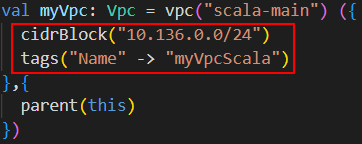
\includegraphics[width=0.5\columnwidth]{case_study/vpc_b_methods} 
  \captionof{figure}{vpc methods}
\end{center}\mbox{}\\
Once such a lambda will be invoked inside the vpc function itself, these methods will be executed, but on which builder?\\
We already mentioned the fact that inside the vpc function a context instance of the VpcArgs.Builder is initialized and the \texttt{init} lambda is able to use it as input parameter thanks to the '\texttt{?=>}' operator we have seen.
But how can the actual \texttt{cidrBlock} and \texttt{tags} methods know on which builder they are being invoked?\\
Without surprise, those methods take the \texttt{VpcArgs.Builder} builder as an implicit parameter with the \texttt{using} keyword.\\
This is the signature for the \texttt{cidrBlock} method in the syntactic sugar file named "PulumiBuilderUtilFunctionsForScala.scala":
\begin{lstlisting}[numbers=left, numberstyle=\tiny, numbersep=-5pt, stepnumber=1, linewidth=420pt]
  def cidrBlock(param: String | Output[String]) (using b: cidrBlockOwners): Unit
\end{lstlisting}\mbox{}\\
We can notice that we have once more a curried function.
Anyway, from how we have seen before, the \texttt{cidrBlock} (and analogously for all the other builder methods) is called with just a single set of parentheses.
This is due to the fact that the second parentheses here are taking an implicit parameter, properly marked with the \texttt{using} keyword.\\
The \texttt{param} parameter is, as we have seen in the \hyperref[sssec:union]{Union type} paragraph, a union type.
The \texttt{String | Output[String]} type is defined so since the Pulumi Java APIs for the builders' methods accept bot a String and an Output[String].
Actually, in the Java implementation an overloading of methods is given since the union type of Scala is not available.\\
The second parentheses are taking an implicit parameter \texttt{b} of the type \texttt{cidrBlockOwners}, that is defined as follows:
\begin{lstlisting}[numbers=left, numberstyle=\tiny, numbersep=-5pt, stepnumber=1, linewidth=420pt]
  type cidrBlockOwners = RouteTableRouteArgs.Builder | SubnetArgs.Builder | VpcArgs.Builder
\end{lstlisting}\mbox{}\\
This is a user defined type that I defined to match the builders of all the \text{Args} classes that are interested in having such a parameter to assign on their builder instance.
In fact in the Java APIs of Pulumi we have many different \texttt{Args} classes' builders that want to assign the same parameter (aka. \texttt{cidrBlock}) to their own builder.
I remind that in the AWS EC2 module there are much more builders of the \texttt{Args} classes that define a cidrBlock method, but my syntactic sugar has created the methods for only the classes that I used in the case study.
This choice has been made also for simplicity in presenting the work done, otherwise the \texttt{cidrBlockOwners} type would have been featuring many tens of types.
The fact we used a union type to define this function has two main motivations.
The first is a Scala language constraint that we came across.
Lets say that we wanted to define a function to assign the CIDR block working exclusively for \texttt{VpcArgs.Builder} class.
A definition of such a function would look like:
\begin{lstlisting}[numbers=left, numberstyle=\tiny, numbersep=-5pt, stepnumber=1, linewidth=420pt]
  def cidrBlock(param: String | Output[String]) (using b: VpcArgs.Builder): Unit =
      param match
        case x: String => builder.cidrBlock(x)
        case x: Output[String] => builder.cidrBlock(x)
\end{lstlisting}\mbox{}\\
And now lets define another function that is working for the \texttt{RouteTableRouteArgs.Builder}:
\begin{lstlisting}[numbers=left, numberstyle=\tiny, numbersep=-5pt, stepnumber=1, linewidth=420pt]
  def cidrBlock(param: String | Output[String]) (using b: RouteTableRouteArgs.Builder): Unit =
      param match
        case x: String => builder.cidrBlock(x)
        case x: Output[String] => builder.cidrBlock(x)
\end{lstlisting}\mbox{}\\
First, we can notice that they are actually the same, except for the signature , but such a solution is not going to compile if we try to call the method \texttt{cidrBlock("10.136.0.0/24")} here:
\begin{lstlisting}[numbers=left, numberstyle=\tiny, numbersep=-5pt, stepnumber=1, linewidth=420pt]
  val myVpc: Vpc = vpc("scala-main") ({
    cidrBlock("10.136.0.0/24") \\ ERROR
    tags("Name" -> "myVpcScala")
  },{
    parent(this)
  })
\end{lstlisting}\mbox{}\\
The compiler will tell us that an ambiguous function call is present at the line 2 of this block of code.
This is due to the fact that the functions we defined are curried and their type is \texttt{(String | Output[String]) => (VpcArgs.Builder => Unit)} and \texttt{(String | Output[String]) => (RouteTableRouteArgs.Builder => Unit)} respectively.
When we call \texttt{cidrBlock("10.136.0.0/24")} on the line 2 of the code showed above, we are partially applying the curried function and so the compiler doesn't know which function we are trying to call, since it can't infer the exact function call basing only on a different return type (that is the only difference in the two functions).\\
The second reason is that our \textit{all-in-one} solution is reducing the size of the generated \textit{sugarized} code, since we have just one single method instead of having as many as the builders of the \texttt{Args} classes that require that methods are.\\

Now we are ready to present the entire \texttt{cidrBlock} method:
\begin{lstlisting}[numbers=left, numberstyle=\tiny, numbersep=-5pt, stepnumber=1, linewidth=420pt]
  def cidrBlock(param: String | Output[String]) (using b: cidrBlockOwners): Unit =
    b match
      case builder: RouteTableRouteArgs.Builder =>
        param match
          case x: String => builder.cidrBlock(x)
          case x: Output[String] => builder.cidrBlock(x)
      case builder: SubnetArgs.Builder =>
        param match
          case x: String => builder.cidrBlock(x)
          case x: Output[String] => builder.cidrBlock(x)
      case builder: VpcArgs.Builder =>
        param match
          case x: String => builder.cidrBlock(x)
          case x: Output[String] => builder.cidrBlock(x)
\end{lstlisting}\mbox{}\\
The body of the function is quite simple in its functioning.
It uses the pattern matching to match the correct builder type and then uses pattern matching once more to match the \texttt{param} parameter to a \texttt{String} or an \texttt{Ouput[String]}.
Finally it calls the Java API of Pulumi to set the cidrBlock parameter on the builder instance b.\\
The fact we have duplicated code here is inevitable.
This is the only solution since if we try to split the duplicated code into an helper function, we would fall again in the ambiguous call error presented above.
But since this is automatically generated code, it is not a real problem to have some duplicated code.\\

To have the final picture of all the functioning lets consider this image:
\begin{center}
  \hspace*{-3cm}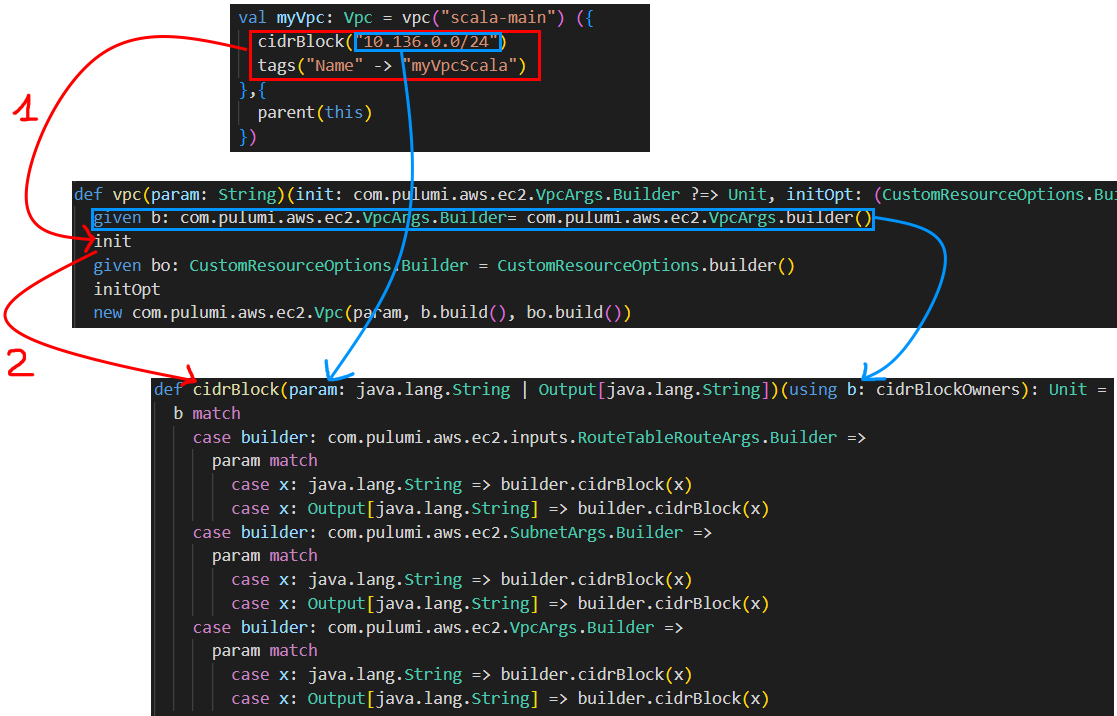
\includegraphics[width=1.4\columnwidth]{case_study/syn-sug-flow} 
  \captionof{figure}{Function calls flow and parameters passing}
\end{center}\mbox{}\\
We can see how the lambda with the calls to our defined methods \texttt{cidrBlock} and \texttt{tags} is passed as the \text{init} parameter of the \textit{sugarized} \texttt{vpc} function.
Inside the \texttt{vpc} function we execute that lambda and so, the \texttt{cidrBlock} method is invoked.\\
In blue we can see from where the parameters of the \texttt{cidrBlock} method are coming from.
The \texttt{String} representing the CIDR block is coming directly from the explicit parameter that we passed,
while the \texttt{VpcArgs} builder is implicitly injected from the compiler since a \textit{given} instance is defined inside the vpc function and the \texttt{b} parameter of the \texttt{cidrBlock} method is marked with \texttt{using}.

\subsubsection{Implicit conversion functions}
\label{sssec:implicit-converion-functions}
On top of this, to boost our syntactic sugar I defined also two extra functions: \texttt{tupleToMap} and \texttt{elemToList}.
The purpose of this functions is to achieve the tricks that I mentioned previously (in the \hyperref[sssec:vpc-creation-scala]{Vpc creation in Scala} and in the the \hyperref[sssec:routetable-creation-scala]{Routetable creation in Scala}) about not needing to explicitly instantiate a singleton Map and a singleton List while passing a single argument to the \texttt{tags} or the \texttt{routes} methods.
The \texttt{tupleToMap} function is implemented like this:
\begin{lstlisting}[numbers=left, numberstyle=\tiny, numbersep=-5pt, stepnumber=1, linewidth=420pt]
  given tupleToMap[A, B]: Conversion[(A, B), Map[A, B]] =
	  (tuple: (A, B)) => Map(tuple)
\end{lstlisting}\mbox{}\\
We can notice that the function that converts our tuple into a singleton Map is based on the Converion class of Scala.
When a suitable argument for the conversion of type (A, B) is found in the code, and a Map[A, B] type is expected, then the compiler will apply the conversion to that type.
This is exactly what happens with our tuple as single parameter passed to the \texttt{tags} method.\\
And the \texttt{elemToList} function is defined in this way instead:
\begin{lstlisting}[numbers=left, numberstyle=\tiny, numbersep=-5pt, stepnumber=1, linewidth=420pt]
  given elemToList[A <: ResourceArgs]: Conversion[A, List[A]] =
	  (elem: A) => List(elem)
\end{lstlisting}\mbox{}\\
The functioning is analogous to \texttt{tupleToMap}, but here we added the extra constraint that A must be a subtype of the \texttt{ResourceArgs} type.
This will prevent undesired too generic conversions that could create problems in the compilation of our program.

\subsection{Functor and Monad implementation for the Output type}
After having introduced the concept of functor and monad in the \hyperref[sssec:functors-monads]{Functor and monads} section, it is here show how the implementation of the monad for the \texttt{Ouput} type has been achieved.\\
Since a monad is also a functor, lets see how \texttt{Functor[Output]} has been implemented.

\subsubsection{Functor implementation}
First a \texttt{Functor} trait has been defined:
\begin{lstlisting}[numbers=left, numberstyle=\tiny, numbersep=-5pt, stepnumber=1, linewidth=420pt]
  trait Functor[F[_]]:
    extension [A](x: F[A])
      def map[B](f: A => B): F[B]
\end{lstlisting}\mbox{}\\
A type \texttt{Output} to be a functor has to implement a map method, that as we have already seen is provided as an extension method.\\
The functor for the \texttt{Output} type is implemented like this:
\begin{lstlisting}[numbers=left, numberstyle=\tiny, numbersep=-5pt, stepnumber=1, linewidth=420pt]
  given Functor[Output] with
    extension [A](oa: Output[A])
      def map[B](f: A => B): Output[B] =
        oa.applyValue(f.asJava)
\end{lstlisting}\mbox{}\\
The implementation of the map method relies on the Java APIs of Pulumi, where the \texttt{applyValue} method from the Output class is provided.\\
The signature of the given method is \texttt{default <U> Output<U> applyValue(Function<T, U> func)}.
We are interested in observing that this method takes a function that transforms a value of a type \texttt{T} in a value of type \texttt{U}, and then it returns an \texttt{Output[U]} value as result.
This signature is exactly the one we need.\\
In fact it is sufficient to pass the function \texttt{f} taken in input from the \texttt{map} invocation and pass it directly to the applyValue method.
To be precise, being \texttt{f} a Scala function, we need to convert it to a Java function before passing it to \texttt{applyValue}.
We achieve this by using the \texttt{.asJava} method from the \texttt{scala.jdk.FunctionConverters.\_} conversion library for Scala.

\subsubsection{Monad implementation}
As for the \texttt{Functor}, the \texttt{Monad} trait has been defined:
\begin{lstlisting}[numbers=left, numberstyle=\tiny, numbersep=-5pt, stepnumber=1, linewidth=420pt]
  trait Monad[F[_]] extends Functor[F]:
    // The unit value for a monad
    def pure[A](x: A): F[A]

    extension [A](x: F[A])
      // The fundamental composition operation
      def flatMap[B](f: A => F[B]): F[B]
      // The `map` operation can now be defined in terms of `flatMap`
      def map[B](f: A => B) = x.flatMap(f.andThen(pure))
\end{lstlisting}\mbox{}\\
A monad, to be called so, must define a \texttt{pure} function.
I remind that such a method puts a value inside a context.\\
Then the \texttt{faltMap}, that is the other method required from a monad, is defined as an extension method.\\
The \texttt{map} method instead can be now be redefined using \texttt{flatMap}.
This is letting us not depend any more on the \texttt{.applyValue} from the Pulumi libraries for Java, because we can now use flatMap to achieve the desired result.\\
The monad for the \texttt{Output} type is implemented in this way:
\begin{lstlisting}[numbers=left, numberstyle=\tiny, numbersep=-5pt, stepnumber=1, linewidth=420pt]
  given Monad[Output] with
    def pure[A](x: A): Output[A] = Output.of(x)
    extension [A](oa: Output[A])
      def flatMap[B](f: A => Output[B]): Output[B] = oa.apply(f.asJava)
\end{lstlisting}\mbox{}\\
The pure method is defined with the Java's Pulumi method \texttt{of}.
It simply boxes the value in an \texttt{Output} context.\\
The \texttt{flatMap} function for the \texttt{Output[A]} type is implemented using the \texttt{.apply} function offered from the Pulumi's Java Output class.
The \texttt{apply} function has a different type from the \texttt{applyValue} one.
As we have seen above, \texttt{applyValue} is matching with the type of \texttt{map}, while the \texttt{apply} has the following signature: \texttt{<U> Output<U> apply(Function<T, Output<U>> func)}.
Since the function passed to \texttt{apply} takes a type \texttt{T} as input and returns a type \texttt{Output<U>} as result, and the whole \texttt{apply} returns an \texttt{Output<U>}, we have a perfect type match with the \texttt{flatMap} signature.
In fact it will suffices us to use \texttt{apply.(f.asSJava)} to have the work done.

Thanks to this implementation we are able, as we have seen in the \hyperref[sssec:subnets-creation]{Subnets creation in Scala} paragraph, to use map on \texttt{availabilityZonesNames()} to apply some logic upon the extracted zone names.
In fact, \texttt{availabilityZonesNames()} is Output[GetAvailabilityZonesResult], and being now Output a monad, the map function is supported.
We succeeded in getting rid of the \texttt{.pulumiall} method.

\subsection{Automatic code generation for the syntactic sugar}
The generation of the syntactic sugar code required the following 2 passages:
\begin{itemize}
  \item Analyze the source code of Pulumi's Java APIs for AWS EC2 in order to infer information about the constructors of the various resources and the builders' methods present in the Builder of each \texttt{Args} class
  \item Use the extracted information to automatically generate the \textit{sugarized} code
\end{itemize}
The first step has been quite straight forward with the aid of the JavaParser library.\\
The second step has been more problematic.
As a first attempt, I tried to use the metaprogramming features offered from the new Scala 3 Macros to create the autogenerated code in the form of an \gls{abstract syntax tree} (AST).
This solution was potentially promising, since Scala also offers the opportunity to convert these ASTs in code and vice versa at compile time, and so telling us about any error at compile time.
The problem encountered is that once we defined the macros for a new type (like \texttt{cidrBlockOwners}), such a type wasn't available at compile time for the other code.
In other words, the types generated through the macro, cannot be referenced in the same project since the whole compilation must finish before having the chance to use the brand new types.\\
Another option was represented by Scalameta, a library to read, analyze, transform and generate Scala programs, but it isn't compatible with Scala 3, and so I had no chance to use it.
If the support for Scala 3 will be added to Scalameta, it should be considered as a better approach for the generation of the syntactic sugar code in the future.\\
So, for the second step, a standard \textit{naive} approach has been adopted.
The auto-generated code is created with a program that inserts the piece of information extracted from the analysis of the Java APIs with Javaparser into a template for the PulumiBuilderUtilFunctionsForScala and the PulumiUtilFunctionsForScala functions.
The generated code can then be exported as a library and included into the dependencies of the building tool used in the Pulumi Scala project.

\subsubsection{Pulumi Java APIs libraries inspection with JavaParser}
Since the code of the project for the inspection is quite verbose (Javaparser is a Java library) and not particularly interesting for the final objective of the thesis, I won't report any of the code here.
I'll limit to describe the steps that are done to infer the required information from the Java libraries for Pulumi.

\paragraph{Non Args and Args classes}
In the Java APIs of Pulumi we have two kind of files (and so classes).
The firsts are the \textbf{non} ...\texttt{Args} files, that are those files that contain the API for the constructor of a given resource.
The second kind of files are represented by the \texttt{Args} files.
Thes classes contains the Builder definition of the respective class and the APIs of the builders' methods used to pass the arguments of the resource while building it with an instance of a builder
For example, we have the Vpc.java file and the VpcArgs.java files.

\paragraph{DirExplorer}
The first class that I defined is \texttt{DirExplorer}. This class has the objective to find all the files in a given directory (and the files in the subdirectories), letting us apply some extra logic during its traverse.
We'll be using such a class in a \texttt{InferInformation} class to extract all the names of the files of our interest.\\

\paragraph{InferInformation}
In the \texttt{InferInformation} class we have 3 methods:
\begin{description}
  \item[listBuilderMethods] is the function that opens every ...\texttt{Args.java} file and, after having parsed an AST of such file, will save all the methods of its builder in a data structure that we'll introduce soon
  \item[listConstructorMethods] is the function that opens every \textbf{non} ...\texttt{Args.java} and, after having parsed the corresponding AST, checks if a public constructor for the given resource is available. In such a case it will add the name of the class to a List that represents all the constructors that should be generated for our syntactic sugar code.
  \item[listFiles] is an helper function for the other two methods that just provides the file names of the classes inspected
\end{description}
The data structure used to store the builders' method has the type \texttt{Map[String, (String, LinkedList[String])]}.
The key of this map is the name of every different builders' method encountered during the parsing of the files.
The value of the Map is a list of all the ...\texttt{Args} classes that contain such a method.
In other worlds, for each method we map all the classes that define such a function.
The entry for the \texttt{cidrBlock} method on the Map (parsing all the files) looks like this:
\begin{verbatim}
cidrBlock: [
  DefaultNetworkAclEgressArgs,
  DefaultNetworkAclIngressArgs,
  DefaultRouteTableRouteArgs,
  GetSubnetArgs,
  GetSubnetPlainArgs,
  GetVpcArgs,
  GetVpcPeeringConnectionArgs,
  GetVpcPeeringConnectionPlainArgs,
  GetVpcPlainArgs,
  NetworkAclEgressArgs,
  NetworkAclIngressArgs,
  RouteTableRouteArgs,
  NetworkAclRuleArgs,
  SubnetArgs,
  SubnetCidrReservationArgs,
  VpcArgs,
  VpcIpv4CidrBlockAssociationArgs
]
\end{verbatim}
Among all this values, we can find the \texttt{VpcArgs}, \texttt{RouteTableRouteArgs} and \texttt{SubnetArgs} that we used in our implementation, and to which we passed a CIDR block using the \texttt{cidrBlock} method.\\
With the information achieved we are now ready to fill in the templates and generate the syntactic sugar for the Scala APIs of Pulumi.

\subsubsection{Raw automatic syntactic sugar code generation}
The class that generates all the code is quite simple.
A Java \texttt{FileWriter} will take care of writing all the strings that represents our code in the PulumiBuilderUtilFunctionsForScala.scala and PulumiUtilFunctionsForScala.scala files.\\
We have two functions, named \texttt{writeContentForBuilders} and \texttt{writeContentForConstructors} that will write all the \textit{various pieces} of generated code into the files using the \texttt{FileWriter}.
With \textit{various pieces} I refer to the generated types for the methods of the builders, the imports, the conversion functions, ecc.\\
Finally we have a bunch of functions that fill the various templates to generate the \textit{various pieces} of code.
These functions are: \texttt{generateTypes}, \texttt{generateBuilderMethods}, \texttt{generateConstructors}, and \texttt{generateImplicitConversionFunctions}.
To have an idea of how the filling of a template works lets consider the \texttt{generateConstructors} function:
\begin{center}
  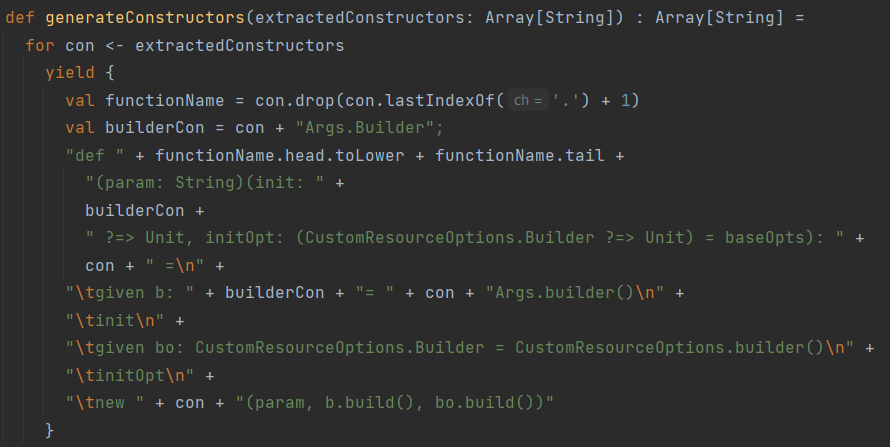
\includegraphics[width=1\columnwidth]{case_study/template_gen} 
  \captionof{figure}{Constructors generation}
\end{center}\mbox{}\\
The template is filled with the variables that represent the name of the constructors, and this is done for each constructor that has been found.\\
Since also the other functions are similar to this one, won't be reported here.

\subsubsection{The automatically generated syntactic sugar code}
Since the generated files contains many hundreds of lines of code, I'll report here only some samples of each file.\\

\paragraph{PulumiBuilderUtilFunctionsForScala}
First we have some default imports:
\begin{center}
  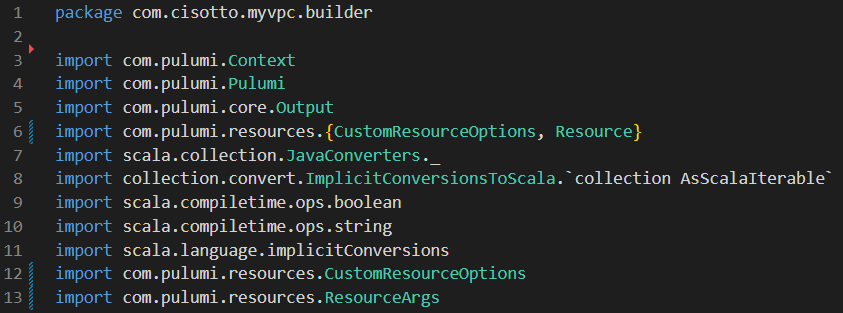
\includegraphics[width=1\columnwidth]{case_study/build_imports} 
  \captionof{figure}{Default import}
\end{center}\mbox{}\\
Then we have some all the generated union types, that look like:
\begin{center}
  \hspace*{-3cm}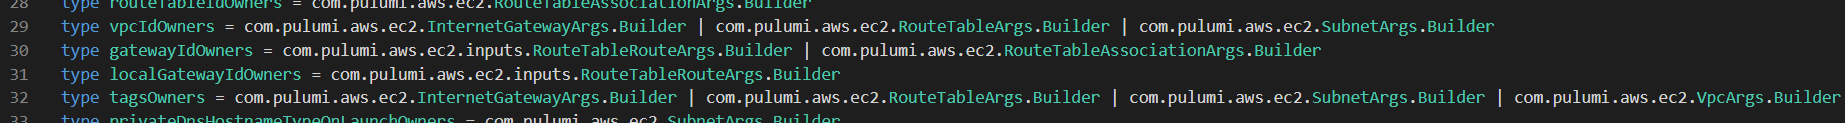
\includegraphics[width=1.5\columnwidth]{case_study/generated_union_types} 
  \captionof{figure}{Generated union types}
\end{center}\mbox{}\\
The implicit conversion functions are then printed:
\begin{center}
  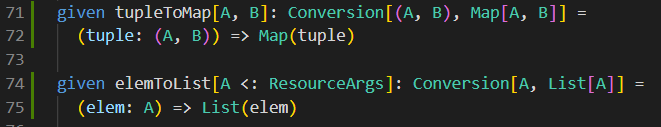
\includegraphics[width=1\columnwidth]{case_study/implicit_conv_fun} 
  \captionof{figure}{Implicit conversion functions}
\end{center}\mbox{}\\
Finally we have all the builders' methods that we encountered during our visit of the files with the JavaParser project:
\begin{center}
  \hspace*{-3cm}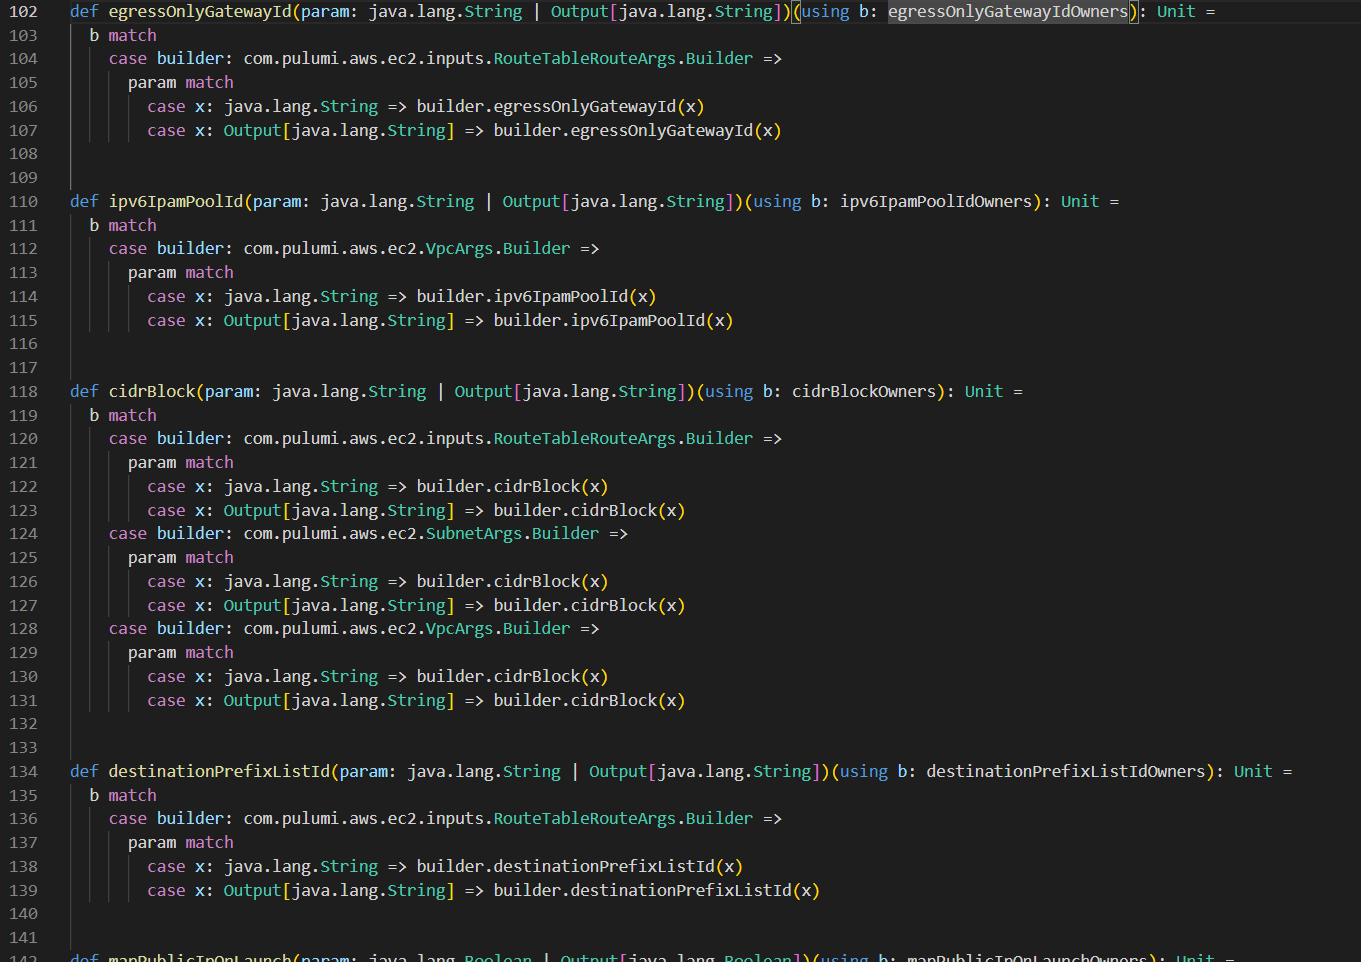
\includegraphics[width=1.4\columnwidth]{case_study/generated_builder_methods} 
  \captionof{figure}{Generated builders' methods}
\end{center}\mbox{}\\

\paragraph{PulumiUtilFunctionsForScala}
Also here we start with some default imports, then we have the baseOpts function and then all the constructors for the various resources:
\begin{center}
  \hspace*{-3cm}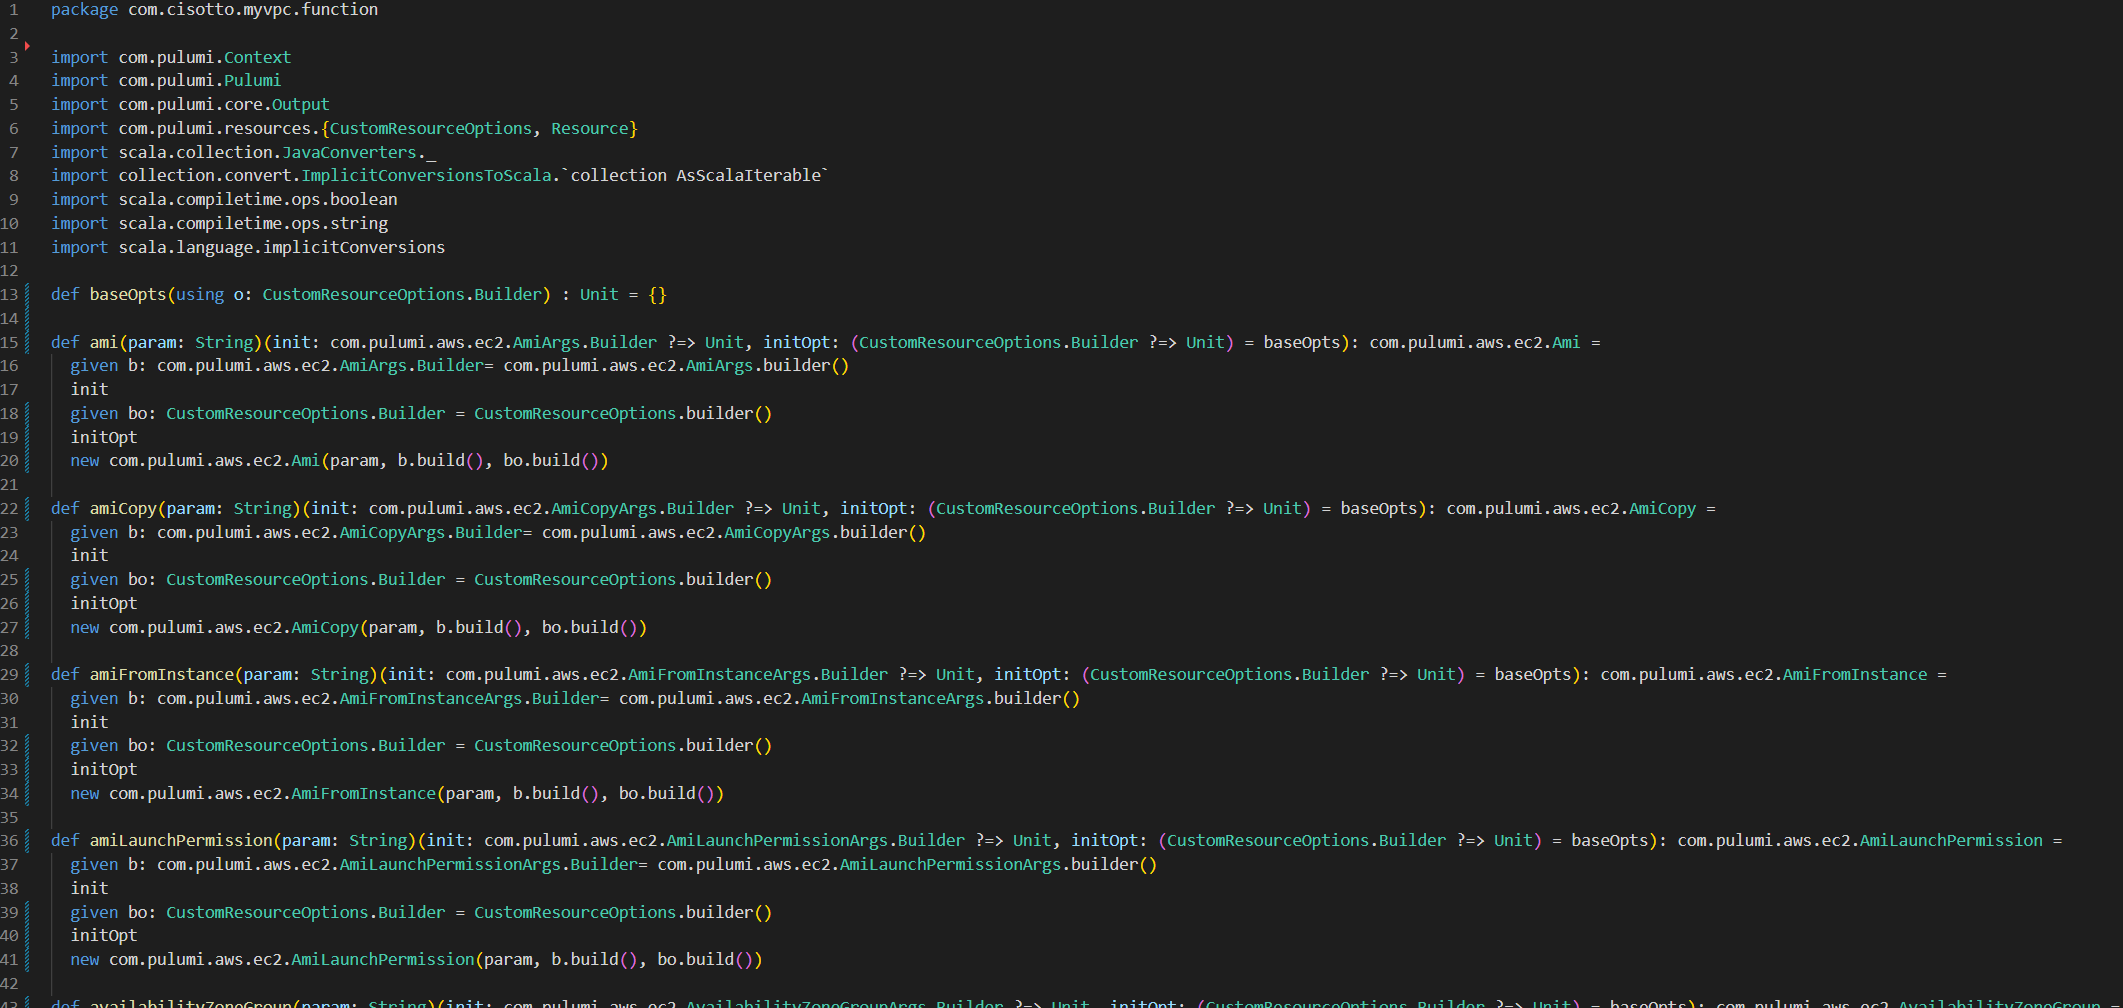
\includegraphics[width=1.4\columnwidth]{case_study/generated_constructors} 
  \captionof{figure}{baseOpts function and generated constructors}
\end{center}\mbox{}\\

\paragraph{Final observations on the generated code}
The builders' methods are really similar to each other, but they are not all following the same exact pattern across the whol AWS EC2 module.
Due to this fact, the generation of the code was affordable for the resources used in the case study, but to cover some corner cases for the rest of the resources some extra work both for the parser and for the algorithm that fills in the template would have been required.
Because of lack of time and since was not the final aim of the thesis to develop a complete support of Scala for all the AWS EC2 module, only the partial support for the used resources has been generated.\\
The constructors, instead, are all similar to each other and a complete support for AWS EC2 has been generated.